\documentclass[a4paper,11pt,twoside]{scrartcl}
\usepackage[T1]{fontenc}
\usepackage{subcaption}
\usepackage[utf8]{inputenc}
\usepackage{ngerman, eucal, mathrsfs, amsfonts, bbm, amsmath, amssymb, stmaryrd,graphicx, array, geometry, color, wrapfig, float, hyperref, epstopdf,gensymb, subcaption}
\geometry{left=25mm, right=15mm, bottom=25mm}
\setlength{\parindent}{0em} 
\setlength{\headheight}{0em} 
\title{Graphentheorie\\ Blatt 3}
\author{Markus Vieth\and Christian Stricker}
\date{\today}
\input{../head/lstlisting.tex}
\usepackage{float}
\usepackage[section]{placeins}
\usepackage{epstopdf}
\usepackage{wrapfig}
\usepackage{caption}
\usepackage{subcaption}
\usepackage{graphicx}
\usepackage{pgfplots}
\usepackage[usenames,dvipsnames,svgnames,table]{xcolor}
\usetikzlibrary{plotmarks}
\usetikzlibrary{patterns}
\usetikzlibrary{decorations.pathmorphing}
\usetikzlibrary{calc}
\usetikzlibrary{shapes}
\newcommand{\coloredcircled}[3][black]{{\large \Large\color{#2}\textcircled {{\small\color{#1}#3}}}}% Circlecolor, Textcolor, text
\newcommand{\ddvec}[2]{\begin{pmatrix}#1\\#2\end{pmatrix}}
\newcommand{\dddvec}[3]{\begin{pmatrix}#1\\#2\\#3\end{pmatrix}}
\newcommand{\longvec}[1]{\overset{\longrightarrow}{#1}}
\newcommand{\eunorm}[1]{\left\lVert#1\right\rVert_2}
\newcommand{\scalar}[2]{\left<#1,#2\right>}\newcommand{\cor}[1]{\textcolor{red}{\textit{#1}}}
\newcommand{\qed}{%
	\begin{flushright}
		q.e.d.
	\end{flushright}%
	}
\begin{document}
\maketitle
\cleardoublepage
\pagestyle{myheadings}
\markboth{Markus Vieth, Christian Stricker}{Markus Vieth, Christian Stricker}

\newpage
\section{Aufgabe 1}
\subsection{a)}

\begin{figure}[H]
	\centering
	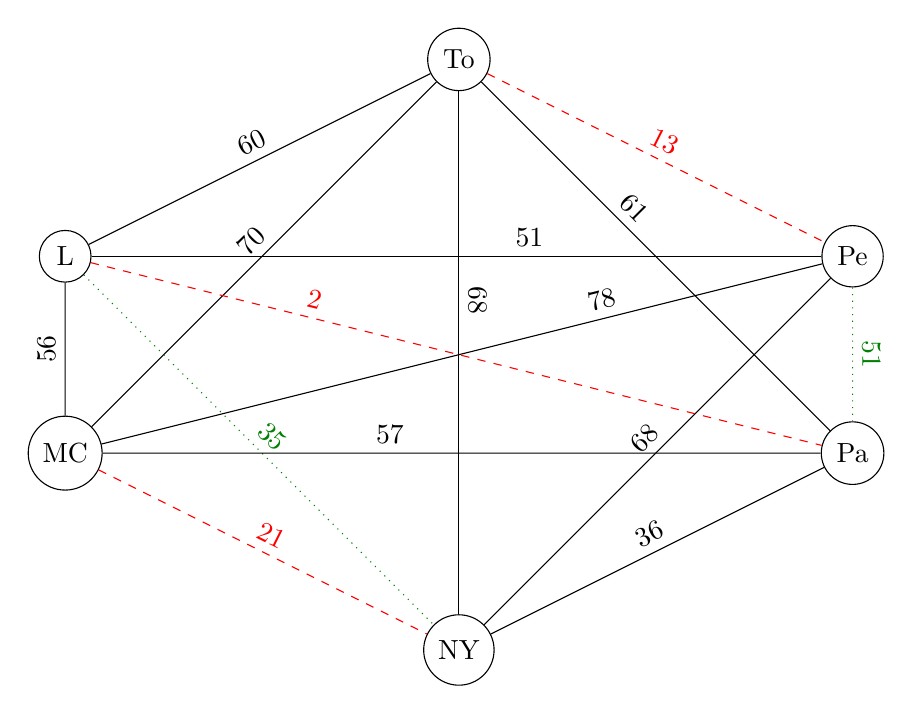
\begin{tikzpicture}[scale=5]
\node[circle, draw=black] at (0,0) (To){To};
\node[circle, draw=black] at (-1,-.5) (L){L};
\node[circle, draw=black] at (1,-.5) (Pe){Pe};
\node[circle, draw=black] at (-1,-1) (MC){MC};
\node[circle, draw=black] at (1,-1) (Pa){Pa};
\node[circle, draw=black] at (0,-1.5) (NY){NY};

\draw (To) -- (L) node [midway, above, sloped] {60};
\draw[color=red, dashed] (To) -- (Pe) node [midway, above, sloped] {13};
\draw (To) -- (MC) node [midway, above, sloped] {70};
\draw (To) -- (NY) node [pos=.4, above, sloped] {68};
\draw (To) -- (Pa) node [pos=.4, above, sloped] {61};

\draw (Pe) -- (L) node [pos=.4, above, sloped] {51};
\draw (Pe) -- (MC) node [pos=.3, above, sloped] {78};
\draw (Pe) -- (NY) node [midway, above, sloped] {68};
\draw[color=Green, dotted] (Pe) -- (Pa) node [midway, above, sloped] {51};

\draw (L) -- (MC) node [midway, above, sloped] {56};
\draw[color=Green, dotted] (L) -- (NY) node [midway, above, sloped] {35};
\draw[color=red, dashed] (L) -- (Pa) node [pos=.3, above, sloped] {2};

\draw[color=red, dashed] (MC) -- (NY) node [midway, above, sloped] {21};
\draw (MC) -- (Pa) node [pos=.4, above, sloped] {57};

\draw (NY) -- (Pa) node [midway, above, sloped] {36};
\end{tikzpicture}
\end{figure}\begin{minipage}{0.5\textwidth}
\begin{description}
	\item[L: ] 60, 51, \coloredcircled{red}{2}, 56, 35
	\item[MC: ] 56, 70, 78, 57, \coloredcircled{red}{21}
	\item[NY: ] \coloredcircled{red}{21}, 35, 68, 68, 36
	\item[Pa: ] 36, 57, \coloredcircled{red}{2}, 61, 51
	\item[Pe: ] 51, 68, 78, 51, \coloredcircled{red}{13}
	\item[To: ] \coloredcircled{red}{13}, 61, 68, 70, 60
\end{description}
\end{minipage}
\begin{minipage}{0.5\textwidth}
\begin{description}
	\item[L, Pa: ] 56, \coloredcircled{Green}{35}, 51, 60, 57, 36, 61, 51
	\item[MC, NY: ] 56, 70, 78, 57, \coloredcircled{Green}{35}, 68, 68, 36
	\item[To, Pe: ] 60, 70, 68, 61, \coloredcircled{Green}{51}, 78, 68, 51
\end{description}
\end{minipage}
Gesamt: $2+21+13+35+51=122$
\subsection{b)}
In jedem Schritt wird die Anzahl der Teilgerüste mindestens halbiert, da der Algorithmus für jedes Teilgerüst die minimale Kante zu einem anderen Teilgerüst auswählt und zu Lösung dazunimmt. Im schlimmsten Fall würden immer Teilgerüstpaare entstehen, d.h. das Problem halbiert sich von Phase zu Phase.\\
(Aus DSeA) $\Rightarrow$ eine Tiefe von $O(\log_2(n))$
\subsection{c)}
\begin{figure}[H]
	\centering
	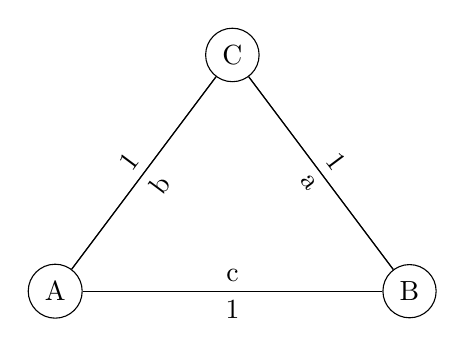
\begin{tikzpicture}[scale=3]
\node[circle, draw=black] at (-.75,-1) (A){A};
\node[circle, draw=black] at (.75,-1) (B){B};
\node[circle, draw=black] at (0,0) (C){C};

\draw (A) -- (B) node [midway, above, sloped] {c};
\draw (A) -- (B) node [midway, below, sloped] {1};

\draw (B) -- (C) node [midway, below, sloped] {a};
\draw (B) -- (C) node [midway, above, sloped] {1};

\draw (C) -- (A) node [midway, below, sloped] {b};
\draw (C) -- (A) node [midway, above, sloped] {1};
\end{tikzpicture}
\caption{Beispiel}
\end{figure}
\begin{tabular}{clcl}
	Knoten& A &nimmt Kante& c\\
	\textacutedbl& B &\textacutedbl& a\\
	\textacutedbl& C &\textacutedbl& b
\end{tabular}\\
\begin{tabular}{ll}
Minimalster Spannbaum laut Algorithmus:& $|a,b,c| = 3$\\
Minimalster Spannbaum wirklich:& $|a,b|$ oder $|b,c|$ oder $|c,a|$ mit Länge $2$.
\end{tabular}
\subsection{d)}
Um die geforderte Laufzeit zu erreichen nutzen wir 2 Phasen:
\begin{description}
	\item[1. Phase] Reduziere die Größe des Graphen mit Bor\r{u}vka
	\item[2. Phase] Finde MST mit Prim
\end{description}
\paragraph{Phase 1}
Da Bor\r{u}vka für eine Iteration, $O(|E|)$ dauert und wir eine Laufzeit von $O(|E|\log\log|V|)$ erreichen wollen, können wir uns $O(\log\log|V|)$ Iterationen von den sonst $O(\log|V|)$ vielen leisten. Die Anzahl der Bäume nach der i-ten Iteration beträgt $O\left(\frac{|V|}{2^{i}}\right)$, nach $\log\log|V|$ Iterationen also $O\left(\frac{|V|}{2^{\log\log|V|}}\right) = O\left(\frac{|V|}{\log|V|}\right)$ viele.\\
$\Rightarrow$ Laufzeit Phase 1 $\in O(|E|\log\log|V|)$\\
\paragraph{Phase 2}
Wir betrachten im Folgenden den Graphen $G'=(V',E')$ in welchem die Bäume zu Überknoten zusammengeführt wurden. Nun wenden wir Prim mit einem Fibonacci-Heap auf diesen Graphen $G'$ an. Somit finden wir die Kanten, mit denen wir die kleinen Bäume aus Phase 1 zu einem großen MST verbinden können. Die Laufzeit beträgt somit \[O\left( |E'| + |V'|\log|V'| \right) \subset\footnote{Abschätzung nach oben}~~O\left( |E| + \frac{|V|}{\log|V|}\log|V| \right) = O\left( |E| + |V| \right)\]
\paragraph{Laufzeit}
\[ O(|E|\log\log|V|) + O\left( |E| + |V| \right) = O(|E|\log\log|V|) \]
\paragraph{Korrektheit}
Da beide Algorithmen immer die kleinst mögliche Kante hinzufügen, erzeugt auch der zusammengesetzte Algorithmus den MST\footnote{siehe \href{https://github.com/Gusser93/DSeA-Vorlesung/blob/master/Vorlesung.pdf}{DSeA}, Schnitt-Lemma, Seite 67}.
%\begin{tikzpicture}
%\begin{axis}[xmin=0, ymin=0, zmin=0, view={20}{33}, xlabel={$|E|$},ylabel={$|V|$}]
%
%\addplot3[raw gnuplot,colormap/redyellow, mesh,shader=interp, samples y=1000] gnuplot {
%	set samples 20,20;
%	set isosamples 20,20;
%	log2(x) = log(x)/log(2);
%	splot [0:1000] [0:1000] x+y;
%};
%\addlegendentry{2. Phase};
%\addplot3[raw gnuplot,colormap/viridis, mesh,shader=interp, samples y=1000] gnuplot {
%	set samples 20,20;
%	set isosamples 20,20;
%	log2(x) = log(x)/log(2);
%	splot [0:1000] [0:1000] x*(log2(log2(y)));
%};
%\addlegendentry{1.Phase};

%\addplot3[raw gnuplot,thick, black,shader=interp, samples y=1000] gnuplot {
%	set samples 20,20;
%	set isosamples 20,20;
%	set parametric;
%	log2(x) = log(x)/log(2);
%	f(x) = x*log(log2(x))/(log(log2(x)) - log(2));
%	splot [t=0:500] f(t), t, f(t);
%};
%\addlegendentry{Phase};
%\end{axis}
%\end{tikzpicture}
\end{document}